\documentclass[11pt,a4paper]{article}
\usepackage{geometry}
\geometry{margin=1.5cm}
\usepackage{multicol}
\usepackage{tikz}
\usetikzlibrary{angles,quotes}

\setlength{\parindent}{0pt}
\setlength{\columnsep}{1cm}

 \pagenumbering{gobble} 

% ---- Consistent styles (labels inside angle arcs) ----
\tikzset{
  ang/.style = {
    draw,
    angle radius=10mm,
    angle eccentricity=0.6, % label sits inside the arc
    pic text options={inner sep=0.8pt, fill=white, text=black}
  },
  rt/.style  = {draw, fill=black!10, angle radius=6mm}
}

\begin{document}

\begin{center}
    {\LARGE \textbf{Triangles Review}}\\[6pt]
\end{center}

\begin{multicols}{4}

%---------------- Q1 ----------------
\textbf{1.}
\begin{center}
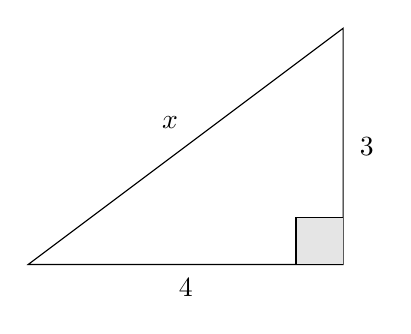
\begin{tikzpicture}[scale=1]
\coordinate (A) at (0,0);
\coordinate (B) at (4,0);
\coordinate (C) at (4,3);
\draw (A)--(B)--(C)--cycle;
\node at (2,-0.3){4};
\node at (4.3,1.5){3};
\node at (1.8,1.8){$x$};
\pic [rt] {right angle = A--B--C};
\end{tikzpicture}
\end{center}

%---------------- Q2 ----------------
\textbf{2.}
\begin{center}
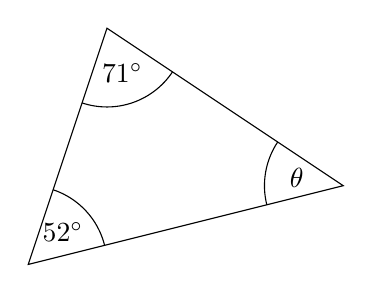
\begin{tikzpicture}[scale=1]
\coordinate (A) at (0,0);
\coordinate (B) at (4,1);
\coordinate (C) at (1,3);
\draw (A)--(B)--(C)--cycle;
  \pic [ang, "$52^\circ$"] {angle = B--A--C};
  \pic [ang, "$71^\circ$"] {angle = A--C--B};
  \pic [ang, "$\theta$"] {angle= C--B--A};
\end{tikzpicture}
\end{center}

%---------------- Q3 (changed to right-angled trig, missing side) ----------------
\textbf{3.}
\begin{center}
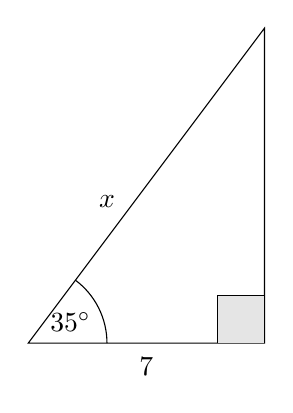
\begin{tikzpicture}[scale=1]
\coordinate (A) at (0,0);
\coordinate (B) at (3,0);
\coordinate (C) at (3,4);
\draw (A)--(B)--(C)--cycle;
\node at (1.5,-0.3){7};       % given adjacent
\node at (1.0,1.8){$x$};      % unknown opposite
\pic [rt] {right angle = A--B--C};
\pic [ang, "$35^\circ$"] {angle = B--A--C}; % angle at A
\end{tikzpicture}
\end{center}

%---------------- Q4 ----------------
\textbf{4.}
\begin{center}
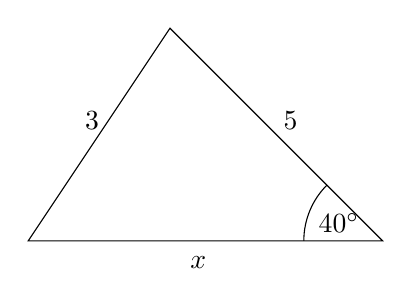
\begin{tikzpicture}[scale=0.9]
\coordinate (A) at (0,0);
\coordinate (B) at (2,3);
\coordinate (C) at (5,0);
\draw (A)--(B)--(C)--cycle;
\node at (0.9,1.7){3};
\node at (3.7,1.7){5};
\node at (2.4,-0.3){$x$};
\pic [ang, "$40^\circ$"] {angle = B--C--A};
\end{tikzpicture}
\end{center}

%---------------- Q5 ----------------
\textbf{5.}
\begin{center}
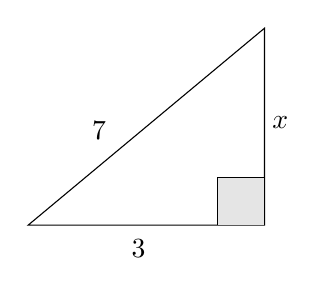
\begin{tikzpicture}[scale=1]
\coordinate (A) at (0,0);
\coordinate (B) at (3,0);
\coordinate (C) at (3,2.5);
\draw (A)--(B)--(C)--cycle;
\node at (1.4,-0.3){3};
\node at (3.2,1.3){$x$};
\node at (0.9,1.2){$7$};
\pic [rt] {right angle = A--B--C};
\end{tikzpicture}
\end{center}

\vspace{8em}

%---------------- Q6 ----------------
\textbf{6.}
\begin{center}
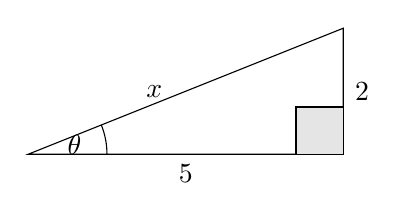
\begin{tikzpicture}[scale=0.8]
\coordinate (A) at (0,0);
\coordinate (B) at (5,0);
\coordinate (C) at (5,2);
\draw (A)--(B)--(C)--cycle;
\node at (2.5,-0.3){5};
\node at (5.3,1){2};
\node at (2,1){$x$};
\pic [rt] {right angle = A--B--C};
\pic [ang, "$\theta$"] {angle = B--A--C};
\end{tikzpicture}
\end{center}

%---------------- Q7 ----------------
\textbf{7.}
\begin{center}
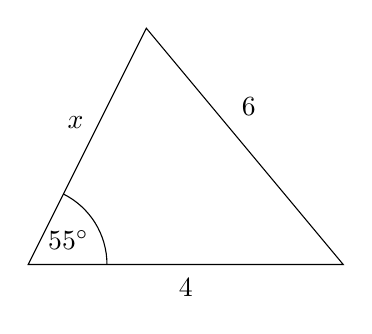
\begin{tikzpicture}[scale=1]
\coordinate (A) at (0,0);
\coordinate (B) at (4,0);
\coordinate (C) at (1.5,3);
\draw (A)--(B)--(C)--cycle;
\node at (2,-0.3){4};
\node at (2.8,2){6};
\node at (0.6,1.8){$x$};
\pic [ang, "$55^\circ$"] {angle = B--A--C};
\end{tikzpicture}
\end{center}

%---------------- Q8 ----------------


\textbf{8.}
\begin{center}
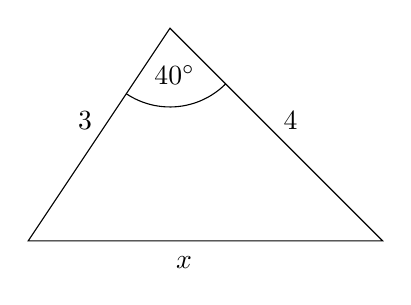
\begin{tikzpicture}[scale=0.9]
\coordinate (A) at (0,0);
\coordinate (B) at (2,3);
\coordinate (C) at (5,0);
\draw (A)--(B)--(C)--cycle;
\node at (0.8,1.7){3};
\node at (3.7,1.7){4};
\node at (2.2,-0.3){$x$};
\pic [ang, "$40^\circ$"] {angle = A--B--C};
\end{tikzpicture}
\end{center}

%---------------- Q9 ----------------
\textbf{9.}
\begin{center}
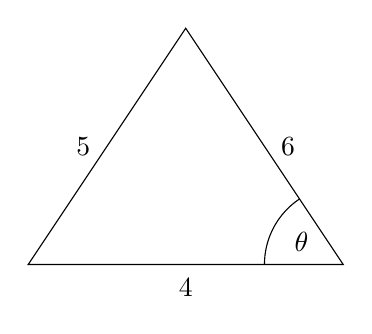
\begin{tikzpicture}[scale=1]
\coordinate (A) at (0,0);
\coordinate (B) at (4,0);
\coordinate (C) at (2,3);
\draw (A)--(B)--(C)--cycle;
\node at (2,-0.3){4};
\node at (0.7,1.5){5};
\node at (3.3,1.5){6};
\pic [ang, "$\theta$"] {angle = C--B--A};
\end{tikzpicture}
\end{center}

%---------------- Q10 ----------------
\textbf{10.}
\begin{center}
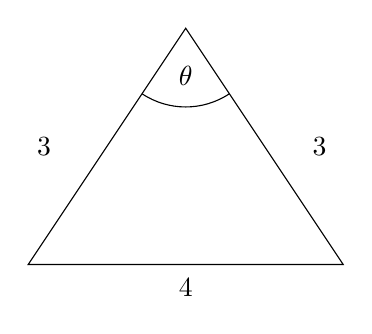
\begin{tikzpicture}[scale=1]
\coordinate (A) at (0,0);
\coordinate (B) at (4,0);
\coordinate (C) at (2,3);
\draw (A)--(B)--(C)--cycle;
\node at (2,-0.3){4};
\node at (0.2,1.5){3};
\node at (3.7,1.5){3};
\pic [ang, "$\theta$"] {angle = A--C--B};
\end{tikzpicture}
\end{center}

\vspace{8em}

%---------------- Q11 ----------------

\textbf{11.}
\begin{center}
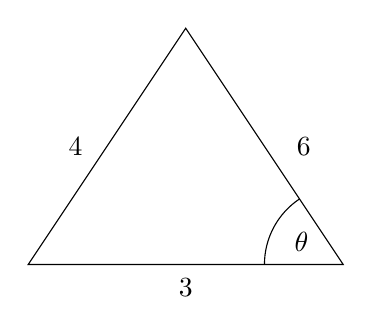
\begin{tikzpicture}[scale=1]
\coordinate (A) at (0,0);
\coordinate (B) at (4,0);
\coordinate (C) at (2,3);
\draw (A)--(B)--(C)--cycle;
\node at (2,-0.3){3};
\node at (0.6,1.5){4};
\node at (3.5,1.5){6};
\pic [ang, "$\theta$"] {angle = C--B--A};
\end{tikzpicture}
\end{center}

%---------------- Q12 (changed to right-angled trig, missing hypotenuse) ----------------
\textbf{12.}
\begin{center}
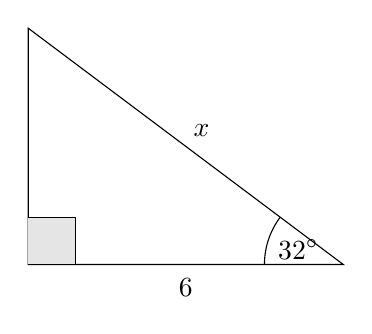
\begin{tikzpicture}[scale=1]
\coordinate (A) at (0,0);
\coordinate (B) at (4,0);
\coordinate (C) at (0,3);
\draw (A)--(B)--(C)--cycle;
\node at (2,-0.3){6};              % given adjacent (AB)
\node at (2.2,1.7){$x$};           % unknown hypotenuse (BC)
\pic [rt] {right angle = B--A--C}; % right angle at A
\pic [ang, "$32^\circ$"] {angle = C--B--A}; % angle at B
\end{tikzpicture}
\end{center}

%---------------- Q13 ----------------
\textbf{13.}
\begin{center}
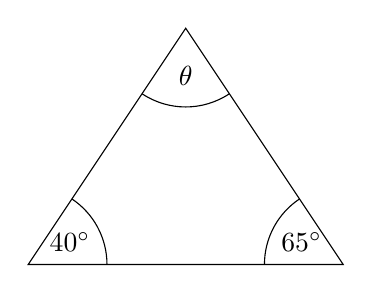
\begin{tikzpicture}[scale=1]
\coordinate (A) at (0,0);
\coordinate (B) at (4,0);
\coordinate (C) at (2,3);
\draw (A)--(B)--(C)--cycle;
\pic [ang, "$40^\circ$"] {angle = B--A--C};
\pic [ang, "$65^\circ$"] {angle = C--B--A};
\pic [ang, "$\theta$"] {angle = A--C--B};
\end{tikzpicture}
\end{center}

%---------------- Q14 ----------------
\textbf{14.}
\begin{center}
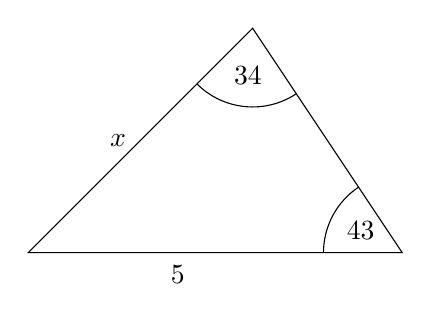
\begin{tikzpicture}[scale=0.95]
\coordinate (A) at (0,0);
\coordinate (B) at (5,0);
\coordinate (C) at (3,3);
\draw (A)--(B)--(C)--cycle;
\node at (2,-0.3){5};
\node at (1.2,1.5){$x$};
\pic [ang, "$43$"] {angle = C--B--A};
\pic [ang, "$34$"] {angle = A--C--B};
\end{tikzpicture}
\end{center}

%---------------- Q15 ----------------
\textbf{15.}
\begin{center}
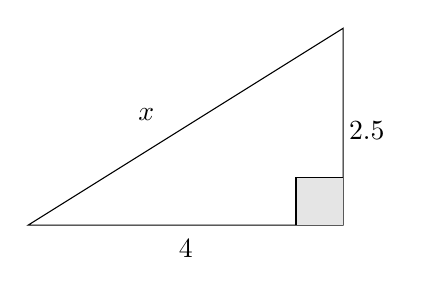
\begin{tikzpicture}[scale=1]
\coordinate (A) at (0,0);
\coordinate (B) at (4,0);
\coordinate (C) at (4,2.5);
\draw (A)--(B)--(C)--cycle;
\node at (2,-0.3){4};
\node at (4.3,1.2){2.5};
\node at (1.5,1.4){$x$};
\pic [rt] {right angle = A--B--C};
\end{tikzpicture}
\end{center}

\vspace{10em}

%---------------- Q16 ----------------
\textbf{16.}
\begin{center}
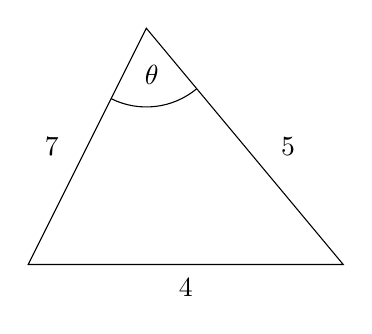
\begin{tikzpicture}[scale=1]
\coordinate (A) at (0,0);
\coordinate (B) at (4,0);
\coordinate (C) at (1.5,3);
\draw (A)--(B)--(C)--cycle;
\node at (2,-0.3){4};
\node at (0.3,1.5){7};
\node at (3.3,1.5){5};
\pic [ang, "$\theta$"] {angle = A--C--B};
\end{tikzpicture}
\end{center}

%---------------- Q17 (changed to right-angled trig, missing angle) ----------------
\textbf{17.}
\begin{center}
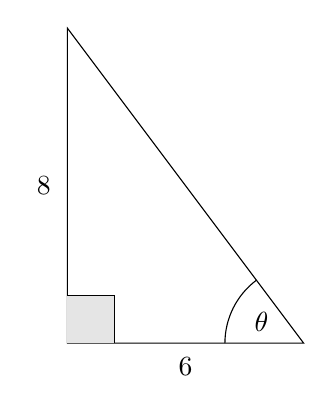
\begin{tikzpicture}[scale=1]
\coordinate (A) at (0,0);
\coordinate (B) at (3,0);
\coordinate (C) at (0,4);
\draw (A)--(B)--(C)--cycle;
\node at (1.5,-0.3){6};  % adjacent (AB)
\node at (-0.3,2){8};    % opposite (AC)
\pic [rt] {right angle = B--A--C};
\pic [ang, "$\theta$"] {angle = C--B--A}; % find the acute angle at B
\end{tikzpicture}
\end{center}

%---------------- Q18 ----------------


\textbf{18.}
\begin{center}
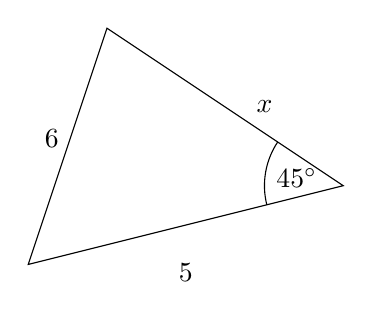
\begin{tikzpicture}[scale=1]
\coordinate (A) at (0,0);
\coordinate (B) at (4,1);
\coordinate (C) at (1,3);
\draw (A)--(B)--(C)--cycle;
\node at (2,-0.1){5};
\node at (0.3,1.6){6};
\node at (3.0,2){$x$};
\pic [ang, "$45^\circ$"] {angle = C--B--A};
\end{tikzpicture}
\end{center}

%---------------- Q19 (changed to right-angled trig, missing side) ----------------
\textbf{19.}
\begin{center}
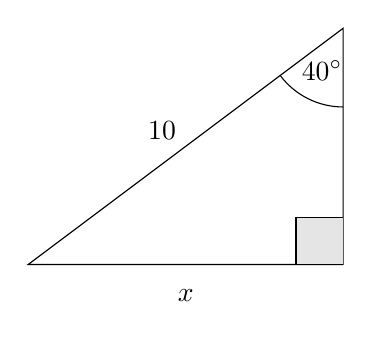
\begin{tikzpicture}[scale=1]
\coordinate (A) at (0,0);
\coordinate (B) at (4,0);
\coordinate (C) at (4,3);
\draw (A)--(B)--(C)--cycle;
\node at (2.0,-0.4){$x$};        % unknown base (AB)
\node at (1.7,1.7){10};         % given hypotenuse (AC)
\pic [rt] {right angle = A--B--C};
\pic [ang, "$40^\circ$"] {angle = A--C--B}; % angle at C
\end{tikzpicture}
\end{center}

%---------------- Q20 ----------------
\textbf{20.}
\begin{center}
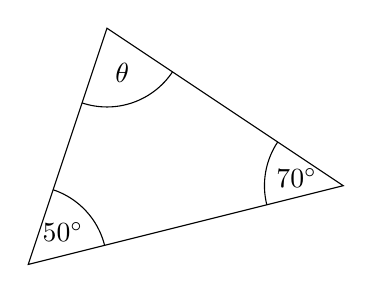
\begin{tikzpicture}[scale=1]
\coordinate (A) at (0,0);
\coordinate (B) at (4,1);
\coordinate (C) at (1,3);
\draw (A)--(B)--(C)--cycle;
\pic [ang, "$50^\circ$"] {angle = B--A--C};
\pic [ang, "$70^\circ$"] {angle = C--B--A};
\pic [ang, "$\theta$"] {angle = A--C--B};
\end{tikzpicture}
\end{center}

\end{multicols}
\end{document}